% !TEX TS-program = Xelatex
% !TEX encoding = UTF-8 Unicode

\documentclass[UTF8]{ctexart}
\usepackage{amsmath}
\usepackage[bottom]{footmisc}
\usepackage{geometry}
\usepackage{graphicx}
\usepackage{figsize}
\usepackage[separate-uncertainty = true,per-mode=symbol]{siunitx}
\usepackage{tabu}
\usepackage{wasysym}
\geometry{left=0.7in,right=0.7in,bottom=0.7in,top=0.7in}

\title{实验九:刚体定轴转动}
\author{朱寅杰 1600017721}
\date{2017年11月24日}

\begin{document}

\maketitle
根据转动定律我们推出当砝码下落的加速度$a\ll g$,即$2h\ll gt^2$时,成立关系式
\[
mgr-M_{\mu}\doteq\frac{2hI}{rt^2}
\]
式中$h=\SI{85.20}{\cm}$为砝码下落的高度,使用卷尺测出。卷尺的允差为\SI{1.2}{\mm},计算不确定度得到$h=\SI{85.20(7)}{\cm}$。$t$为砝码从静止落地用时,使用停表测量。停表的精度为\SI{0.01}{\s}。$r$为转子上绕绳的半径,作为转动时的力臂,使用游标卡尺测量,允差为\SI{.002}{\cm}。
\subsection{固定$r$,拟合$m$与$t$的关系}
固定$r=\SI{2.484}{\cm}$,则有\begin{equation}t^{-2}=\frac{gr^2}{2hI}m-\frac{rM_{\mu}}{2hI}\end{equation}
将$m$从\SI{5}{\g}增加到\SI{35}{\g},分别测量$t$的数值,计算出$t^{-2}$的数值与不确定度,并对$t^{-2}-m$作线性回归。数据记录如下表:
\begin{center}
\noindent
\begin{tabu} to \linewidth {X[c,-1]|X[c,-10] X[c,-10] X[c,-10] X[c,-10] X[c,-10] X[c,-10] X[c,-10]}
\hline
$m$/g	&5.00	&10.05	&15.01	&19.98	&25.06	&30.09	&35.11\\
\hline
$t$/s	&16.63	&11.34	&9.07	&7.91	&6.97	&6.43	&5.88\\
	&16.28	&11.15	&9.22	&7.88	&7.00	&6.37	&5.90\\
	&16.38	&11.41	&9.04	&7.91	&7.03	&6.38	&5.88\\
\hline
$\bar{t}$/s	&16.43	&11.30	&9.11	&7.90	&7.00	&6.39	&5.89\\
$\sigma_{\bar{t}}$/s	&0.104	&0.078	&0.056	&0.010	&0.017	&0.041	&0.007\\
\hline
$\bar{t}^{-2}/\SI{e-3}{\per\second\squared}$	&3.70	&7.83	&12.05	&16.02	&20.4	&24.5	&28.8\\
$\sigma_{t^{-2}}$/\SI{e-4}{\per\second\squared}	&0.47	&1.09	&1.49	&0.47	&1.04	&3.17	&0.89\\
\hline
\end{tabu}
\end{center}
计入$t^{-2}$的不确定度,使用计算机进行回归并自动合成斜率与截距的不确定度得到\[t^{-2}=\SI{8.314(35)e-1}{\per\second\squared\per\kg}\times m-\SI{4.95(66)e-4}{\per\second\squared},r=\num{.99995}\]
从而算出$I=\SI{4.27(2)e-3}{\kg\m\squared}$,$M_{\mu}=\SI{1.45(19)e-4}{\N\m}$。

拟合的直线见附图。由于线性十分好,转动定律推出的关系式(1)得到了验证。

\subsection{固定$m$,拟合$r$与$t$的关系}
固定$m=\SI{19.87}{\g}$,则有
\begin{equation}\frac{1}{t^2r}=\frac{mg}{2hI}r-\frac{M_{\mu}}{2hI}\end{equation}
将$r$从\SI{1}{\cm}增加到\SI{3}{\cm},分别测量$t$的值,计算出$\frac{1}{t^2r}$的值与不确定度,并对$\frac{1}{t^2r}-r$线性回归。数据记录如下表:
\begin{center}
\noindent
\begin{tabu} to \linewidth {X[c,-1]|X[c,-10] X[c,-10] X[c,-10] X[c,-10] X[c,-10]}
\hline
$r$/cm	&0.991	&1.503	&2.001	&2.484	&3.001\\
\hline
$t$/s	&19.34	&12.96	&9.81	&7.97	&6.56\\
	&19.25	&12.94	&9.97	&8.00	&6.53\\
	&19.28	&12.97	&9.88	&7.91	&6.53\\
\hline
$\bar{t}$/s	&19.29	&12.96	&9.92	&7.96	&6.54\\
$\sigma_{\bar{t}}$/s	&0.058	&0.009	&0.046	&0.026	&0.010\\
\hline
$r^{-1}\bar{t}^{-2}/\si{\m^{-1}\second^{-2}}$	&0.271	&0.396	&0.508	&0.635	&0.779	\\
$\sigma_{r^{-1}t^{-2}}$/\SI{e-3}{\m^{-1}\second^{-2}}	&1.7	&0.7	&4.7	&4.2	&2.8	\\
\hline
\end{tabu}
\end{center}
计入$r^{-1}t^{-2}$的不确定度,使用计算机进行回归并自动合成斜率与截距的不确定度得到\[
\frac{1}{t^2r}=\SI{25.09(40)}{\m^{-2}\s^{-2}}\times r-\SI{0.0194(63)}{\m^{-1}\s^{-2}},r=\num{.99962}
\]
从而有$I=\SI{4.55(7)e-3}{\kg\m^2}$,$M_{\mu}=\SI{1.51(33)e-4}{\N\m}=\SI{1.5(3)e-4}{\N\m}$。
拟合的直线见附图。由于线性十分好,转动定律推出的关系式(2)得到了验证。
\subsection{讨论}
首先要保证$a\ll g$,也就是$t\gg \SI{0.42}{\s}$。这在实验中很好地得到了满足,$a$都在$g$的两百分之一以下,因此对结果的误差也在这个数量级。但是$a$随着$m$与$r$的增大而增大,因此在两组实验中测出的斜率都一定是偏小的,使得转动惯量的结果的计算都偏大了约千分之几。

对拟合直线的线性影响最大的恐怕是阻力矩$M_{\mu}$的稳定性,实验时应避免触动转子,保证各处固定螺丝足够紧,并且滑轮切向与绳子方向对齐,这要求在每次改变$r$时都要对准滑轮。但是阻力矩显然不仅仅取决于螺丝的松紧,容易想象转速较快的时候阻力矩较大,因此所测得的斜率仍然不可避免是偏小的。

绳子水平与否会直接在力矩的计算中相差一个余弦的因子,这是一个较为显著的系统误差。即便每次都用刻度尺立在桌面上丈量绳子的高度来确认开始时绳子平行于桌面,由于绳子绕在转子上有一个高度区间,绳子的水平度依然会有波动。如果允许水平角有百分之一弧度的波动,会在结果中产生$\cos 0.01=0.99995$即十万分之五的偏差。这个偏差还是比较小的。

另一个更为显著的系统误差是对转子半径$r$的估计。使用游标卡尺测出的是没有绕上绳子的转子的直径,在绕上绳子以后,转子等效的半径会变大。特别是当绳子并不能单层地绕在转子上的时候,这个效应更为明显。当$r$较小时更容易发生这样的情况,因此在第二组实验中,这个因素会导致较小的$r$的数值被低估了,导致测得的斜率偏小,转动惯量偏大。比如当$r=\SI{.991}{\cm}$时,实际的$r$可能有\SI{1.05}{\cm},以此类推,最终会使得所测得的斜率偏小2\%到3\%,也就是转动惯量偏大2\%到3\%,这个偏差是非常显著的,比上面分析的因素重要得多。第二次测出的转动惯量比第一次大了6.6\%,这应当是一个主要的原因。
\begin{figure}
\centering
\SetFigLayout{2}{1}
\subfigure[固定$r$,拟合$m$与$t^{-2}$的关系。因变量的不确定度已在图中标出。]{\includegraphics{m-t.eps}} \\
\subfigure[固定$m$,拟合$r$与$1/t^2r$的关系。因变量的不确定度已在图中标出。]{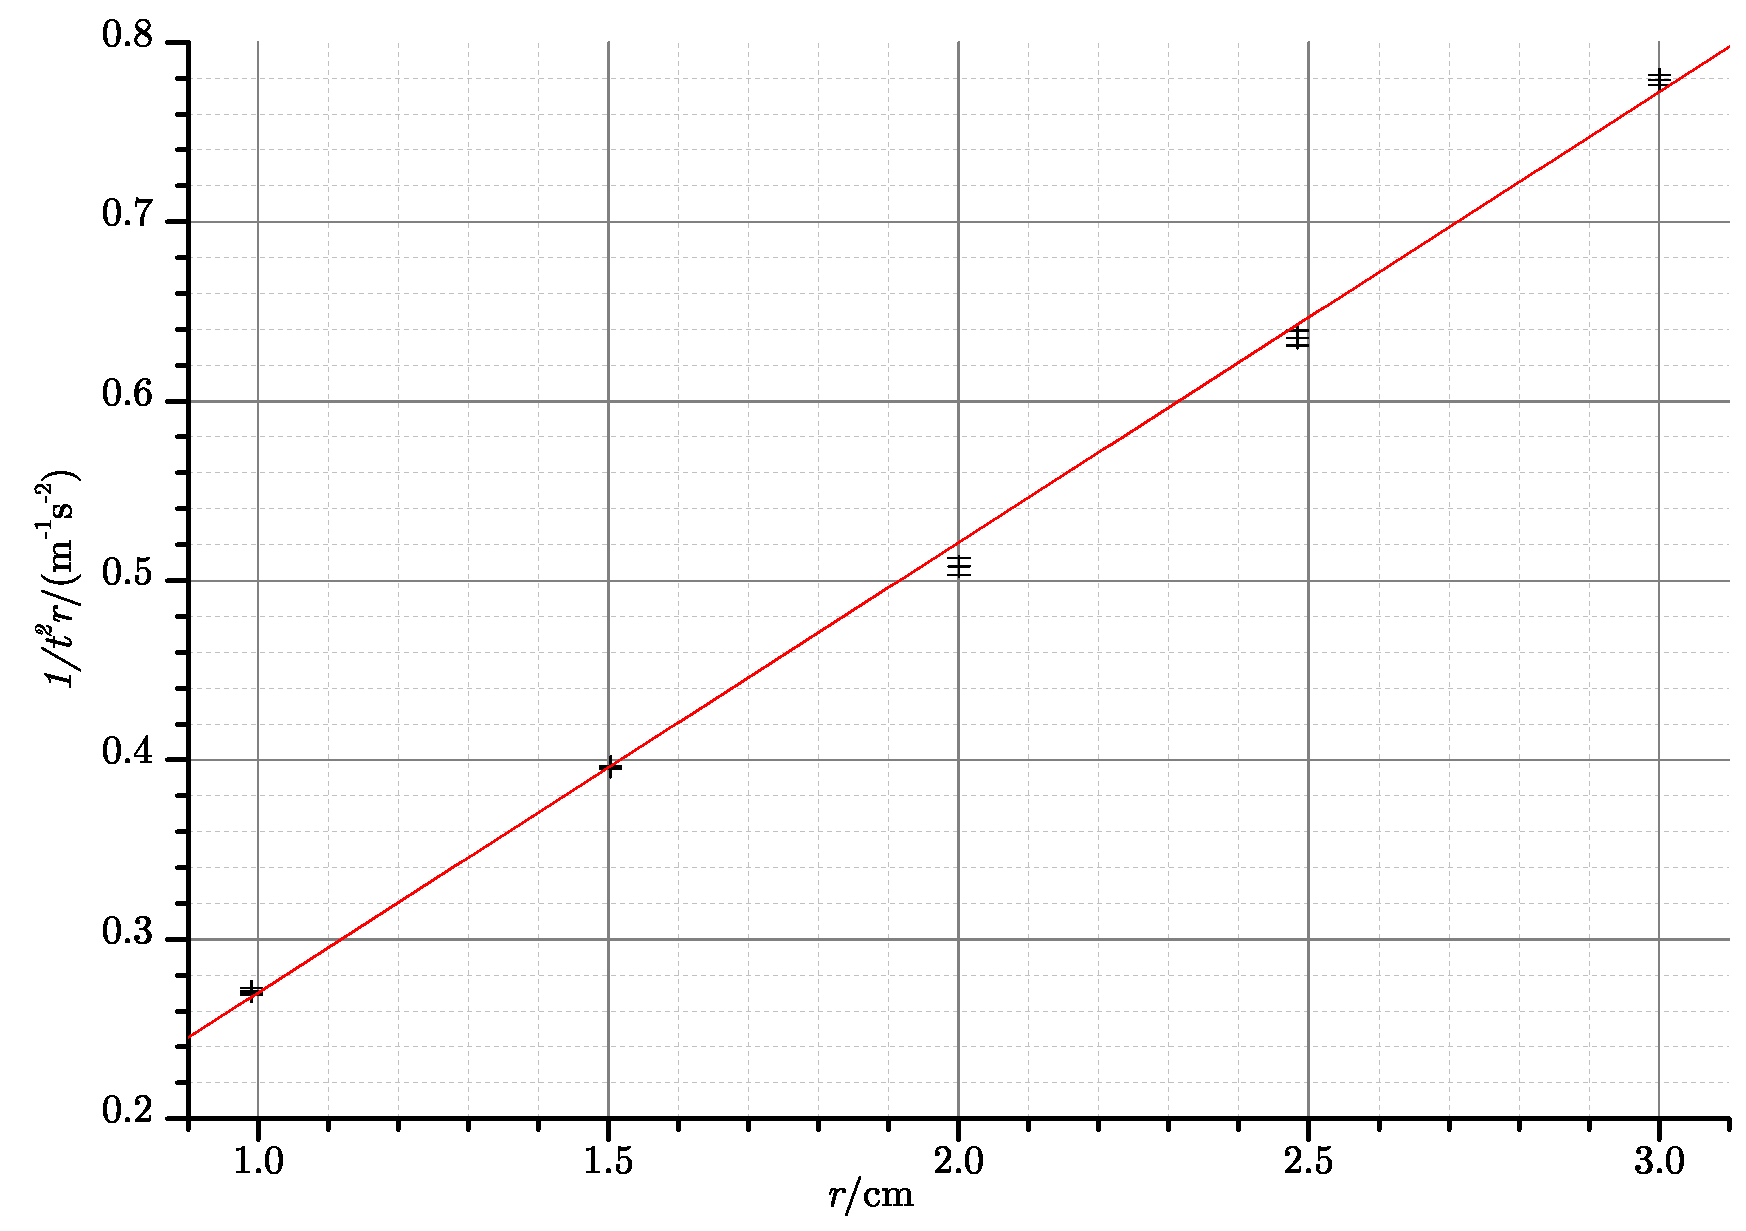
\includegraphics{r-t.eps}} \\
\end{figure}
\end{document} 